The Aggregator produces the Power model's final predictions for an entity by merging the Texter's and Ruler's predictions. After the merge process, the combined predictions are again sorted by confidence, increasing the density of true top predictions. Facts predicted by both Texter and Ruler, should be ranked especially high.

Regarding the merge, however, confidences produced by Ruler and Texter are not necessarily directly comparable, even if they are all from the same range $(0, 1)$. For example, if rule mining was stopped too early, the Ruler's estimations could be systematically too low, because it is missing high-confidence rules for some of its predicted facts. To avoid that in this case actually good predictions are behind less good predictions of the Texter, a weight parameter $\alpha$ is introduced to phase the predictions of Ruler and Texter. Thus, the overall confidence $conf_{Aggregator}$ of a prediction results from the Texter's confidence $conf_{Texter}$ and the Ruler's confidence $conf_{Ruler}$ according to Equation~\ref{eq:4_approach/3_aggregator/conf_aggregator}. Summing up the weighted confidences ensures that facts predicted by both components are ranked particularly highly.

\begin{align}
    conf_{Aggregator} = \alpha \cdot conf_{Texter} + (1 - \alpha) \cdot conf_{Ruler}
    \label{eq:4_approach/3_aggregator/conf_aggregator}
\end{align}

\begin{figure}[t]
    \makebox[\textwidth][c]{
        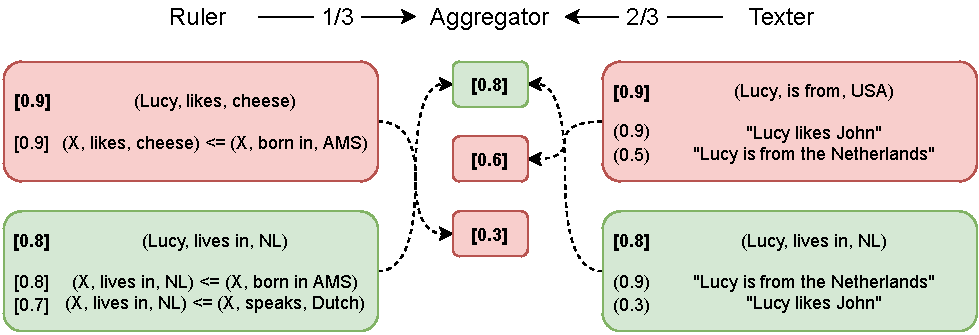
\includegraphics{4_approach/3_aggregator/lucy}
    }
    \caption{Example for Aggregator merging the Ruler's and Texter's predictions with assumed $\alpha = 2/3$, ranking the correct fact predicted by both components the highest - green (red) indicates true (false) positive, [brackets] mark confidences and (parantheses) mark attention values}
    \label{fig:4_approach/3_aggregator/lucy}
\end{figure}

To illustrate the function of the aggregator and recapitulate the Power model's overall approach, Figure~\ref{fig:4_approach/3_aggregator/lucy} demonstrates the inference process by an extended example based on the entity Lucy mentioned in the introductory example in Chapter~\ref{ch:1_introduction}. Given are the sentences "Lucy is from the Netherlands." and "Lucy likes John.", as well as the fact that Lucy was born in Amsterdam. In addition, it shall now be known that Lucy speaks Dutch. The aim is to predict the missig fact $(Lucy, lives~in, Netherlands)$. In this example scenario, calling the Ruler does indeed predict that with a probability of 80\%, since that is the confidence of the strongest rule. Unfortunately, however, the hypothetical graph seems to indicate that 90\% of all individuals born in Amsterdam also like cheese, resulting in an even higher ranked false positive. Thus, in this case the Ruler would achieve precision = 0.5, recall = 1.0, F1 = 0.5 and mAP = 0.5. The situation is similar for the Texter: Again, the explanations for the predicted facts make sense, but the correct fact is only in second place. Finally, the Aggregator merges the Ruler's and Texter's results with an assumed weight factor $\alpha = \frac{2}{3}$, producing the final predictions in which the correct fact $(Lucy, lives~in, Netherlands)$ moved to the top and the mAP increases to 1.0.
